\documentclass[]{article}
%\usepackage{lmodern}
\usepackage{amssymb,amsmath}
\usepackage{ifxetex,ifluatex}
\usepackage{fixltx2e} % provides \textsubscript
\ifnum 0\ifxetex 1\fi\ifluatex 1\fi=0 % if pdftex
  \usepackage[T1]{fontenc}
  \usepackage[utf8]{inputenc}
\else % if luatex or xelatex
  \ifxetex
    \usepackage{mathspec}
    \usepackage{xltxtra,xunicode}
  \else
    \usepackage{fontspec}
  \fi
  \defaultfontfeatures{Mapping=tex-text,Scale=MatchLowercase}
  \newcommand{\euro}{€}
\fi
% use upquote if available, for straight quotes in verbatim environments
\IfFileExists{upquote.sty}{\usepackage{upquote}}{}
% use microtype if available
\IfFileExists{microtype.sty}{%
\usepackage{microtype}
\UseMicrotypeSet[protrusion]{basicmath} % disable protrusion for tt fonts
}{}
\usepackage{graphicx}
\makeatletter
\def\maxwidth{\ifdim\Gin@nat@width>\linewidth\linewidth\else\Gin@nat@width\fi}
\def\maxheight{\ifdim\Gin@nat@height>\textheight\textheight\else\Gin@nat@height\fi}
\makeatother
% Scale images if necessary, so that they will not overflow the page
% margins by default, and it is still possible to overwrite the defaults
% using explicit options in \includegraphics[width, height, ...]{}
\setkeys{Gin}{width=\maxwidth,height=\maxheight,keepaspectratio}
\ifxetex
  \usepackage[setpagesize=false, % page size defined by xetex
              unicode=false, % unicode breaks when used with xetex
              xetex]{hyperref}
\else
  \usepackage[unicode=true]{hyperref}
\fi
\hypersetup{breaklinks=true,
            bookmarks=true,
            pdfauthor={},
            pdftitle={Ethics},
            colorlinks=true,
            citecolor=blue,
            urlcolor=blue,
            linkcolor=magenta,
            pdfborder={0 0 0}}
\urlstyle{same}  % don't use monospace font for urls
\setlength{\parindent}{0pt}
\setlength{\parskip}{6pt plus 2pt minus 1pt}
\setlength{\emergencystretch}{3em}  % prevent overfull lines
\setcounter{secnumdepth}{0}

\title{Ethics}
\date{}

\begin{document}
\maketitle

\subsection{Introduction}\label{introduction}

Ethics is one of philosophy's main specialities. It is also the one that
everyone has already had some familiarity. You already have ethical
beliefs about the following claims:

\begin{enumerate}
\def\labelenumi{\arabic{enumi}.}
\itemsep1pt\parskip0pt\parsep0pt
\item
  Cheating on your partner is never permissible.
\item
  Stealing is never permissible.\\
\item
  It is never permissible to hit someone.
\item
  Lying is never permissible.
\item
  Killing another person is never permissible.
\item
  Abortion is never permissible
\item
  The death penalty is permissible on some occasions.
\item
  Torture is permissible on some occasions.
\item
  Eating meat is never permissible.\\
\item
  I should donate to charity when I can.
\end{enumerate}

You likely agreed with some of these claims, disagreed with others. You
also likely have reasons for why you think some of these claims are
true, others are false. The study of ethics is the study of these
reasons. It is the discipline that tries to determine why certain
actions are allowed, others are prohibited, and others are required. In
particular, ethicists try to adjudicate between a number of theories
about which reasons are relevant for the rightness and wrongness of our
actions. In this brief handout, I will first outline some features of
the reasons that ethicists seek. I will then discuss a challenge to the
very possibility of ever finding reasons that have these features.

\subsection{Ethics and Reasons}\label{ethics-and-reasons}

First, it is important to properly understand the distinction between
what are called \emph{descriptive} and \emph{normative} facts.
Descriptive facts are facts about how the world is. Normative facts are
facts are about how the world should be. Compare the following two
claims:

\begin{enumerate}
\def\labelenumi{\arabic{enumi}.}
\itemsep1pt\parskip0pt\parsep0pt
\item
  ``I am eating sugar''
\item
  ``I should not sugar.''
\end{enumerate}

1 is a descriptive fact. 2 is a normative fact. 2 describes something
that is happening, I am currently eating sugar. It does not say whether
it is good or bad to eat sugar. It just says that I'm doing it. 2, on
the other hand, does not say that I am in fact eating sugar. It says
that I should avoid doing so. 2 can be true even if I never eat sugar. 1
is true only if I am, in fact, eating sugar.

Morality is part of normativity. Moral judgements are about (i) how a
person should act and (ii) what kind of character a person should have.
Consider these two claims:

\begin{enumerate}
\def\labelenumi{\arabic{enumi}.}
\itemsep1pt\parskip0pt\parsep0pt
\item
  ``Sonya is having an affair.''\\
\item
  ``Sonya should not have an affair.''
\end{enumerate}

1 is a descriptive claim. It tell us that Sonya is cheating on her
parter, but it takes no stance on the morality of her action. 2, on the
other hand, is a normative claim. It doesn't say that Sonya is having an
affair. It says that she should not have one. Notice that Sonya might be
a most felicitous person and 2 still true. 2 is telling us something
about what she shouldn't do and not about about what she is doing. Moral
judgements are always like claim 2. They are claims about what actions
we should and should not perform.

In our everyday lives, we expect people to give reasons in support of
their moral judgements and are quick to provide our own. So, someone
might claim that Sonya should not have an affair \emph{because} she
promised to be faithful and having an affair would involve breaking that
promise. Here the reason for 2 is \emph{one shouldn't break a promise.}
Another person might claim that Sonya should remain faithful
\emph{because} having an affair would hurt her partner. Here the reason
for 2 is \emph{one shouldn't hurt another.}

Ethics is the study of these reasons. It tries to determine which
reasons are good ones and which ones are not. So, for instance, some
ethicists deny that it is always wrong to break a promise. If, for
instance, Sonya breaking her promise were the only way to save a
life---admittedly a far flung possibility---some claim that it would be
permissible for her to do so. Many ethicists deny that it is always
wrong to hurt another. Vaccinations might be painful, but many claim we
have an obligation to vaccinate our children even thought doing so is
painful. The point is, Ethics is not so much concerned with giving
reasons for moral judgements as it is concerned with trying to determine
which reasons are adequate, which are not.

If we are going to evaluate moral reasons, distinguish the good reasons
from the bad ones, we need to identify the characteristics of a good
moral reason. These characteristics include:

\begin{itemize}
\itemsep1pt\parskip0pt\parsep0pt
\item
  They are not based on mere emotion, or bias. They are reasons that can
  be evaluated.\\
\item
  They are universal. They apply to everyone regardless of sex, gender,
  race, or culture. If it is wrong to break a promise, then it is wrong
  for everyone, irregardless of who they are, to break a promise.
\item
  They are general. If being F explains why some action, x, is immoral,
  then every other action that is F is also immoral. For instance, if it
  is wrong to cause another pain, then, irrespective of circumstances,
  every action which causes another person pain is immoral. This
  requirement is one of our most helpful. If you really think that it is
  wrong for Sonya to have an affair \emph{merely} because of the pain it
  causes her partner, then you are committed to taking every pain
  causing action as immoral. If you were to then claim that the pain
  involved in vaccinations does not make vaccinations immoral, you would
  be involved in a contradiction and would need to revise one of your
  beliefs.\\
\item
  They override legal considerations. If breaking a promise is immoral,
  then one should keep a promise \emph{even if} it involves breaking a
  law, e.g., refusing to answer a question in court when compelled to by
  a judge. (If you think you should break a promise in this case, you
  don't believe that promise keeping is a real moral obligation.)
\end{itemize}

\subsection{Ethical Theories}\label{ethical-theories}

Ethicists offer different theories about which reasons satisfy these
requirements. These 3 theories offer general claims about the
appropriate reasons for morality. There are three main theories (or
groups of theories.) To introduce you to these theories first look at
this diagram:

\begin{figure}[htbp]
\centering
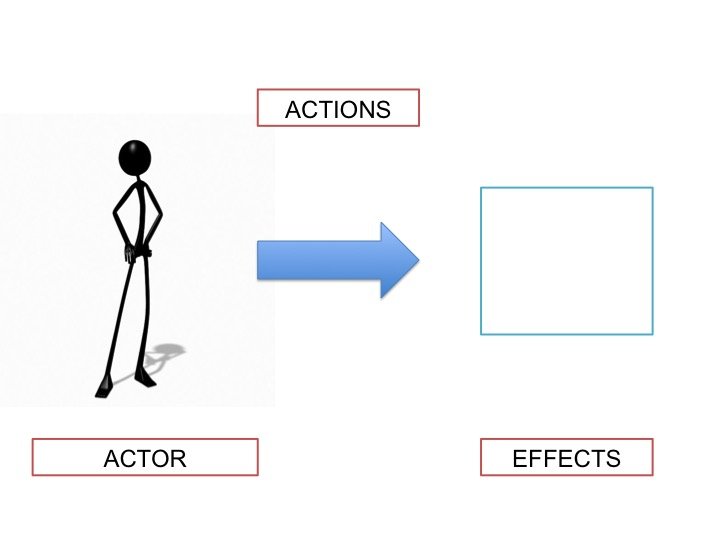
\includegraphics{/Teaching/Examined/Ethics/Slide1.jpg}
\caption{alt text}
\end{figure}

The actor represents each of us. It's the person whose actions will be
evaluated. The arrow represents the various actions people perform,
e.g., walking, punching, complementing, stealing, eating meat, taking
drugs, and so on. The box represents the effects of our various actions.
If punching someone causes them pain, then pain is an effect of
punching. If eating meat were to cause indigestion, then indigestion is
the effect of eating meat.

Our different moral theories explain why actions are moral or immoral
(or neither) by referring to different parts of this diagram. Next week,
we will discuss these theories in detail. I here outline them by way of
introduction:

\begin{enumerate}
\def\labelenumi{\arabic{enumi}.}
\itemsep1pt\parskip0pt\parsep0pt
\item
  \textbf{Consequentialism} claims that the rightness and wrongness of
  an action depends solely on its consequences, on its effects. It says
  that to determine the morality of an action we are to ignore the actor
  side of the diagram. Their motives, intentions, and so on are
  irrelevant. We are also to ignore the arrow part of the diagram. It
  does not matter that the action is a promise breaking, or stealing, or
  murder, etc. All that matters, says the consequentialist, is the
  effects of the action.\\
\item
  \textbf{Deontology} claims that the rightness and wrongness of an
  action depends entirely on the intrinsic nature of the action. It says
  that we are to ignore both the actor in our diagram as well as the
  effects side of the diagram. Neither the motives or character of the
  actor is relevant in determining the morality of their actions.
  Neither is the effects of their actions. Some actions, the
  deontologist claims, are just inherently wrong, e.g., murder, they
  claim, is just inherently wrong.
\item
  \textbf{Virtue Ethics} claims that the rightness and wrongness of an
  action depends entirely on the character of the person performing that
  action, on the actor. Virtue ethics denies that the morality of our
  action has anything to do with the consequences or the intrinsic
  nature of the acts. It depends entirely on whether the action came
  from a person who is virtuous, i.e., it depends entirely on the actor
  side of the diagram.
\end{enumerate}

\subsection{A Challenge to Ethics: Ethical
Relativism}\label{a-challenge-to-ethics-ethical-relativism}

Before discussing these theories, we should address an objection that
attacks not just all three, but any ethical theory. Some have argued
that there are no universal moral truths, truths that hold for all
people and all times. This view, \textbf{moral relativism}, cuts to the
very core of ethics. It claims that we are mistaken when searching for
appropriate reasons for ethical judgements. The relativist claims that
there are no reasons that could serve the role we wish them to play.

The moral relativism we are concerned with says that what's true,
ethically, varies by culture, e.g., causing pain might be immoral in one
culture, but not in a different culture.

Moral relativism is easily misunderstood; it's far more radical than you
might initially think. Distinguish these two claims:

\begin{enumerate}
\def\labelenumi{\arabic{enumi}.}
\itemsep1pt\parskip0pt\parsep0pt
\item
  Culture A believes that abortion is immoral. Culture B believes that
  abortion is morally permissible.
\item
  Abortion \emph{is} morally permissible in Culture B, but not in
  Culture A.
\end{enumerate}

Moral relativism is defending Claim 2, which is much stronger than Claim
1. We might compare Claim 2 to the claim that, say, what's tasty is
relative to a person. Suppose we ask, for instance, whether cilantro is
tasty. A relativist about taste will say that there are no facts about
taste that apply to everyone; cilantro tastes horrible to one person,
but not to another person. If taste is relative, a person can never be
wrong as to whether cilantro is tasty. If they find it tasty, it is
tasty, but to them. If someone claims it is horrible, you cannot claim
they have made a mistake. It will be horrible, but to that person.

Similarly, the moral relativist claims that there are no
\emph{objective} moral standards, standards which apply to all moral
judgements irrespective of where those judgements originated. Morality,
they claim, is quite like taste. If a culture disapproves of an action,
that action really is immoral, not to everyone, but just to members of
the disapproving culture.

Cultural relativism has an important upshot: there are no genuine
cross-cultural moral disagreements. If your culture disapproves of
forcing the elderly to commit suicide, then such force is immoral
\emph{in your culture}. But if another culture approves of forcing the
elderly to kill themselves, you must remain silent. You cannot say that
the other culture has made a mistake, that your culture has the right
policy, and the other has the wrong policy. Your culture's standards are
not theirs, and there is no cross-cultural standard that applies to both
cultures equally that would make one policy immoral, the other moral.

\subsection{The Argument for Cultural
Relativism}\label{the-argument-for-cultural-relativism}

It's useful to have a clear statement of cultural relativism before we
proceed:

\textbf{Claim:} If a culture approves of an action, then that action is
moral for them. If a culture disapproves of an action, then that action
is immoral for them.

For convenience, let us say that this amounts to the claim that there
are no objective moral truths, i.e., there are no general and universal
moral truths (see above for definition)

The argument for Cultural Relativism is called the \emph{Cultural
Differences Argument}. There are different ways of formulating the
argument. You can find one in ch.3.2 of the textbook. I include an
alternative formulation here.

\textbf{Cultural Differences Argument}

\begin{enumerate}
\def\labelenumi{\arabic{enumi}.}
\itemsep1pt\parskip0pt\parsep0pt
\item
  Different cultures have different moral beliefs.
\item
  If different cultures have different moral beliefs, then there are no
  objective moral truths.
\item
  Therefore, there are no objective moral truths.
\end{enumerate}

Premise 1 has a wealth of evidence. The discipline of Anthropology
catalogues and studies the plethora of different cultural differences
across the globe. For some interesting examples, skim
\href{Benedict.pdf}{`Anthropology and the Abnormal'}, by Ruth Benedict.
The study of history provides plenty of other examples. The Callatians,
on the one hand, thought one should eat the bodies of the dead. The
Ancient Greeks, on the other hand, thought the practice abhorrent.

Premise 2 is the crucial claim. Anthropologists report extreme
variations in moral practices across the globe. There does not seem,
they claim, to be any moral belief that is universally shared. This, of
course, might come as a surprise. It would certainly have come as a
surprise to those colonialists who tired to impose their cultural norms
on the peoples whose lands they colonized, often in most horrific and
violent ways.

\subsubsection{Objections to Relativism}\label{objections-to-relativism}

Here I will discuss the main objection to moral relativism. Consult the
textbook for further objections. While the Cultural Differences Argument
is valid, many argue that the second premises is false, and so claim the
argument is not sound.

Premise 2 contains an inference. It says that since moral beliefs vary,
there are no objective moral truths. This inference can be presented as
an argument:

\begin{itemize}
\itemsep1pt\parskip0pt\parsep0pt
\item
  Premise: Moral beliefs vary from culture to culture.
\item
  Conclusion: There are no objective moral facts.
\end{itemize}

Here is a concrete example:

\begin{itemize}
\itemsep1pt\parskip0pt\parsep0pt
\item
  Premise: The Greeks believes that eating the dead was immoral. The
  Callatians believed that eating the dead was their duty.
\item
  Conclusion: It is neither objectively moral or immoral to eat the
  dead.
\end{itemize}

This argument is not valid. The conclusion does not follow from the
premise. The difficulty for the relativist is to supply some premise to
make the argument valid. Few, if any, suggestions seem plausible. The
following general claim would allow us generate a valid argument, but it
is also clearly false:

\begin{itemize}
\itemsep1pt\parskip0pt\parsep0pt
\item
  If cultures disagree about some claim P, then P is neither objectively
  true or objectively false
\end{itemize}

Appeal to this general principle would be a mistake. Notice the
following instances of the principle are clearly absurd:

\begin{itemize}
\itemsep1pt\parskip0pt\parsep0pt
\item
  Premise: The Classical Greeks believed that the Earth was a sphere,
  whereas the ancient Norse believed that the Earth was flat.
\item
  Conclusion: Therefore, the claim that the Earth is a sphere is neither
  objectively right nor objectively wrong.
\end{itemize}

This is a poor argument. The premise is true, but the logic clearly
flawed. The Greeks were right. The Norse were wrong. The sciences
proceed by making and testing hypotheses, rejecting those that are
wrong, accepting those that are right. Before a claim is proved,
scientists regularly are in disagreement. But this disagreement only
shows that they have yet to discover the truth. It does not mean that
there is no truth to discover.

Here is another example:

\begin{itemize}
\itemsep1pt\parskip0pt\parsep0pt
\item
  Premise: The majority of South Koreans believe that climate change is
  caused by human activity, whereas the vast majority of Tanzanians do
  not believe that climate change is caused by human activity.
\item
  Conclusion: Therefore, the claim that climate change is caused by
  human activity is neither objectively true nor objectively false.
\end{itemize}

Again, this is a poor argument. There is a fact of the matter as to
whether humans are causing the Earth to warm. Disagreement between
cultures is no reason to doubt this.

Similarly, the fact cultures disagree on moral issues does not mean
there are no objective moral facts. None of us may have discovered the
truth yet. Or perhaps some culture has discovered the truth and others
are mistaken. But the fact that we have not agreed on what the truth is
does not mean that there is no truth to agree upon. This questionable
inference is central to cultural relativism and should give one pause in
accepting it.

\end{document}
